\documentclass{article}
% \usepackage[utf8]{inputenc}
\usepackage[letterpaper, margin=1in]{geometry}
\usepackage{graphicx}

\begin{document}

\title{Lab 02}
% \label{sec:title}

\section{Prelab}
\label{sec:prelab}

\begin{enumerate}
\item
The early late gate method works by taking samples at least 3 points (A, B, C) of the signal.
If C~$>$~A, then the samples are traveling uphill. If C~$<$~A, then the samples are traveling downhill.
The difference between A and C is proportional to the timing error, and is used in computing
the error. If B is positive, then uphill means sampling happened early and downhill means that
sampling happened late, and visa versa if B is negative. Figure~\ref{fig:earlylate} show examples
of samples being early, late, and on-time.

\begin{figure}[hb]
\centering
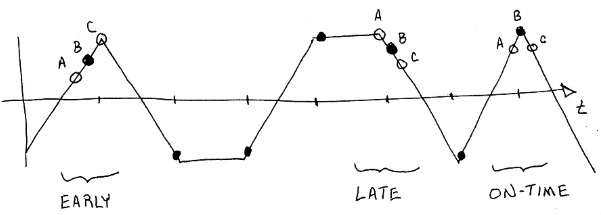
\includegraphics{LateEarlyGate.png}
\caption{Examples of Early-Late Gate}
\label{fig:earlylate}
\end{figure}

\item
Polynomial filter can be used to resample data by estimating abritary samples along the transmitted signal.

\end{enumerate}

\section{Lab}
\label{sec:lab}
\begin{enumerate}
\item[2.] See Figure~\ref{fig:ImpulseResRC}.

\begin{figure}[ht]
\centering
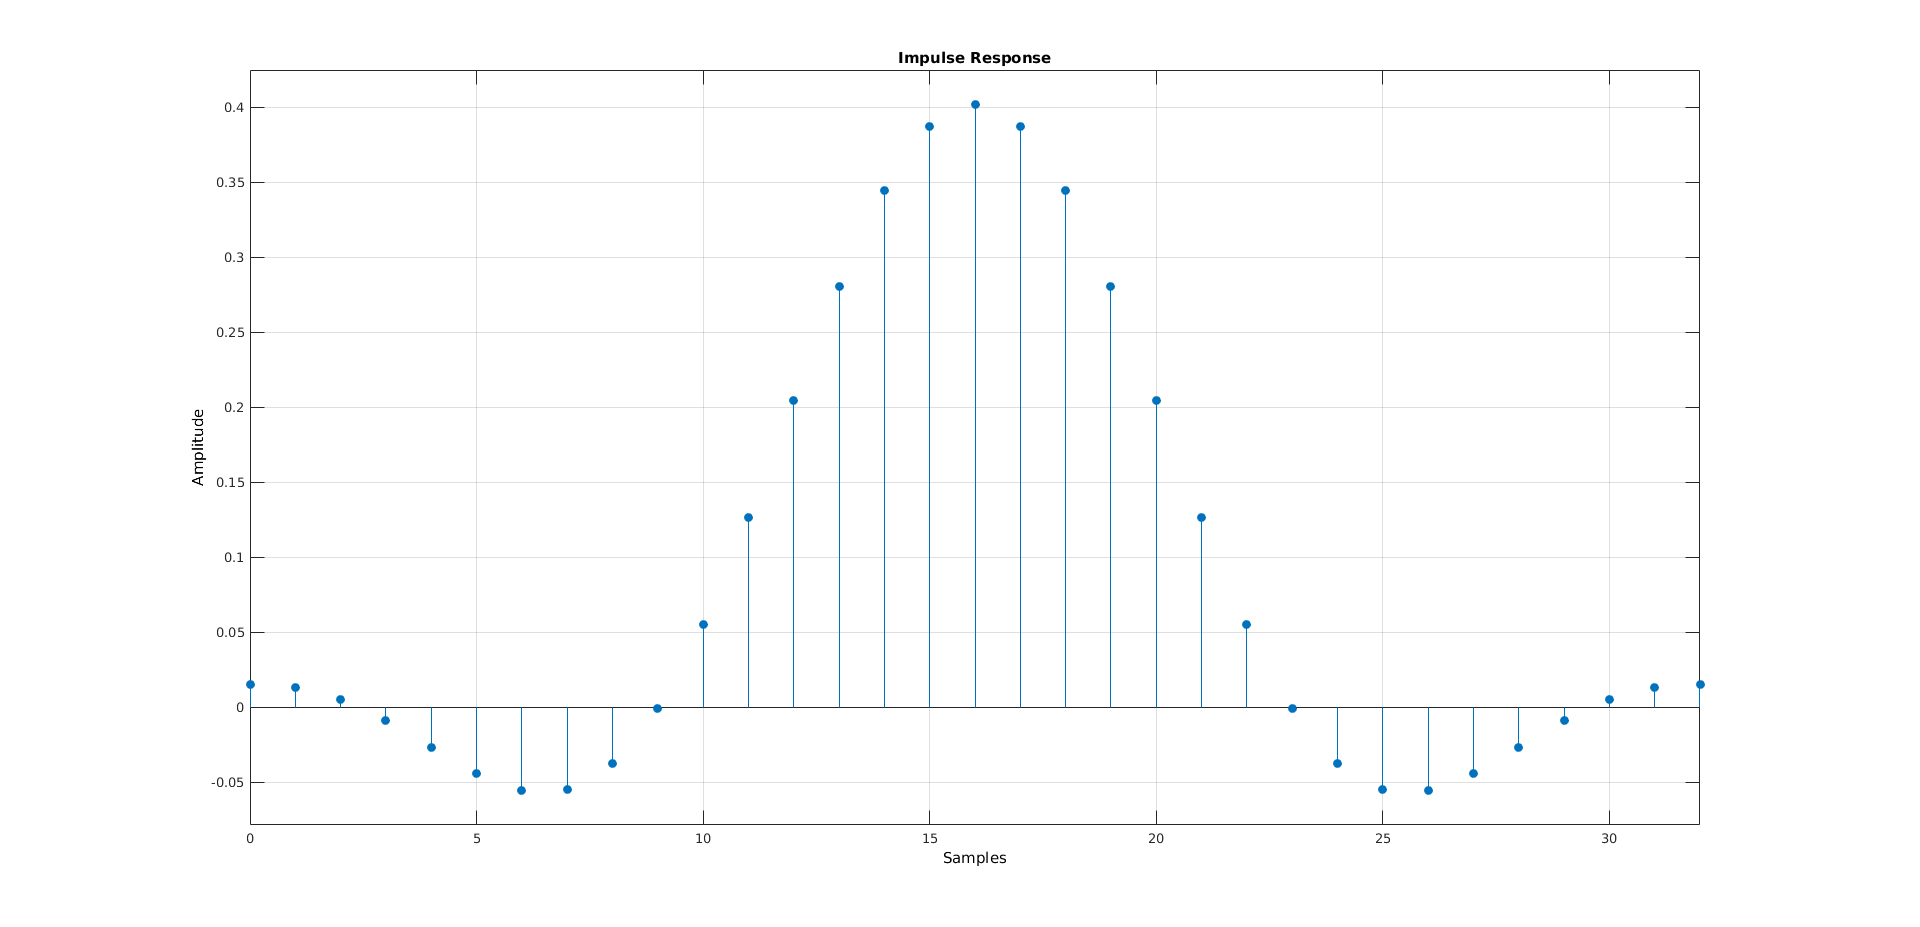
\includegraphics[width=\linewidth]{ImpulseResRC.png}
\caption{Impulse Response of Raised Cosine Function}
\label{fig:ImpulseResRC}
\end{figure}

\item[4.] See Figure~\ref{fig:TransRC}

\begin{figure}[ht]
\centering
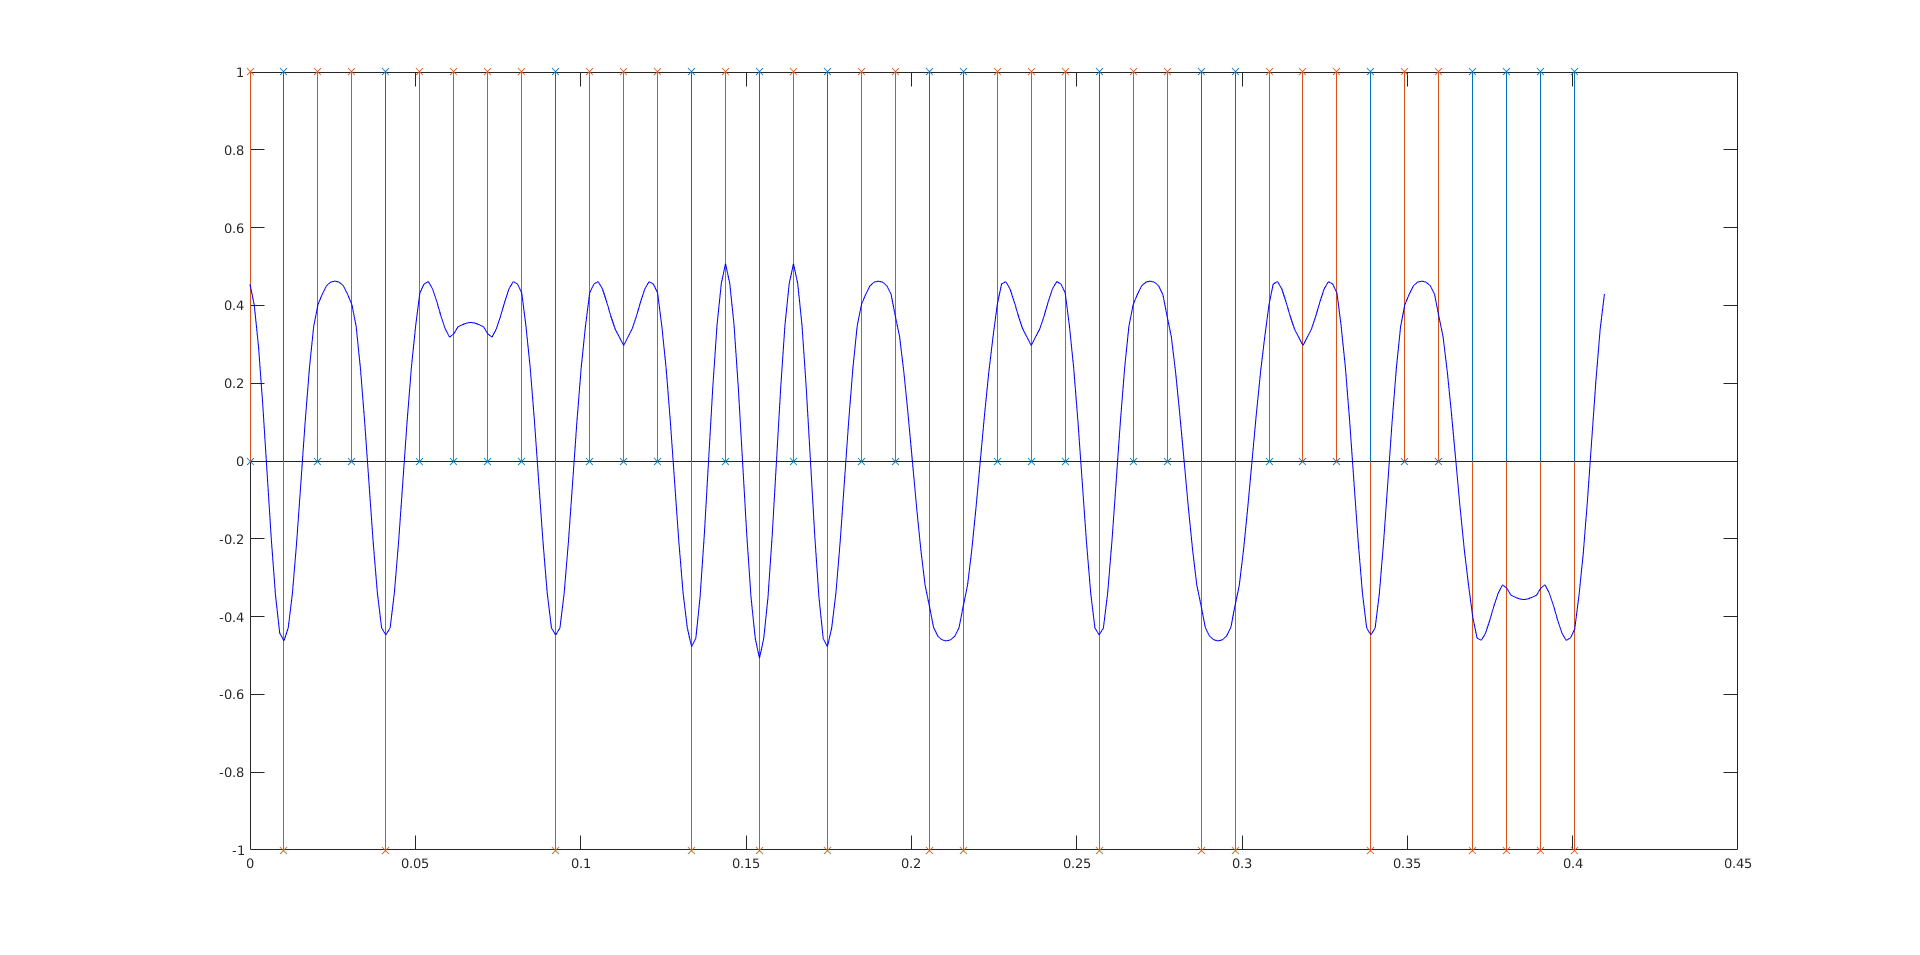
\includegraphics[width=\linewidth]{TransRC.png}
\caption{Input Signal, Modulated Signal, and Filtered Signal}
\label{fig:TransRC}
\end{figure}

\item[5.]
The Effective Data Rate is 778.8 kHz.

\item[7.] See Figure~\ref{fig:RecRC}

\begin{figure}[ht]
\centering
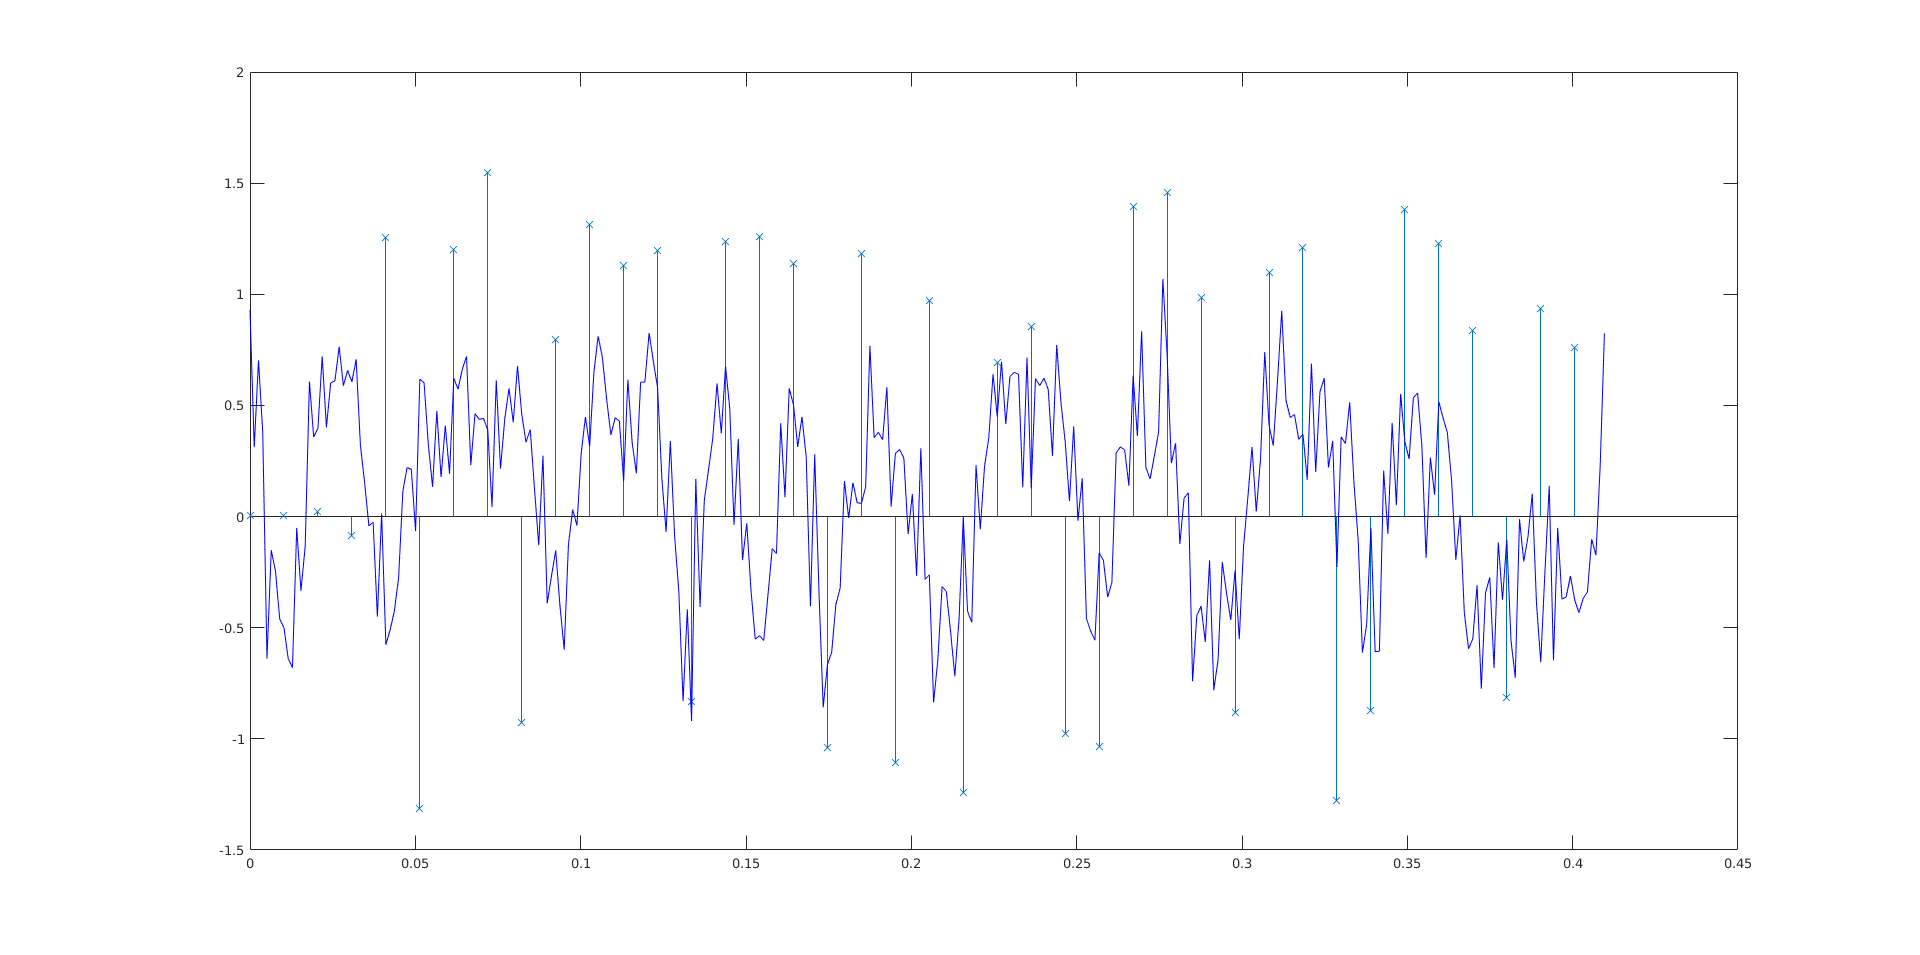
\includegraphics[width=\linewidth]{RecRC.png}
\caption{Input and Output of Receive Filter}
\label{fig:RecRC}
\end{figure}

\item[9.] See Figure~\ref{fig:BERComp}
\begin{figure}[ht]
\centering
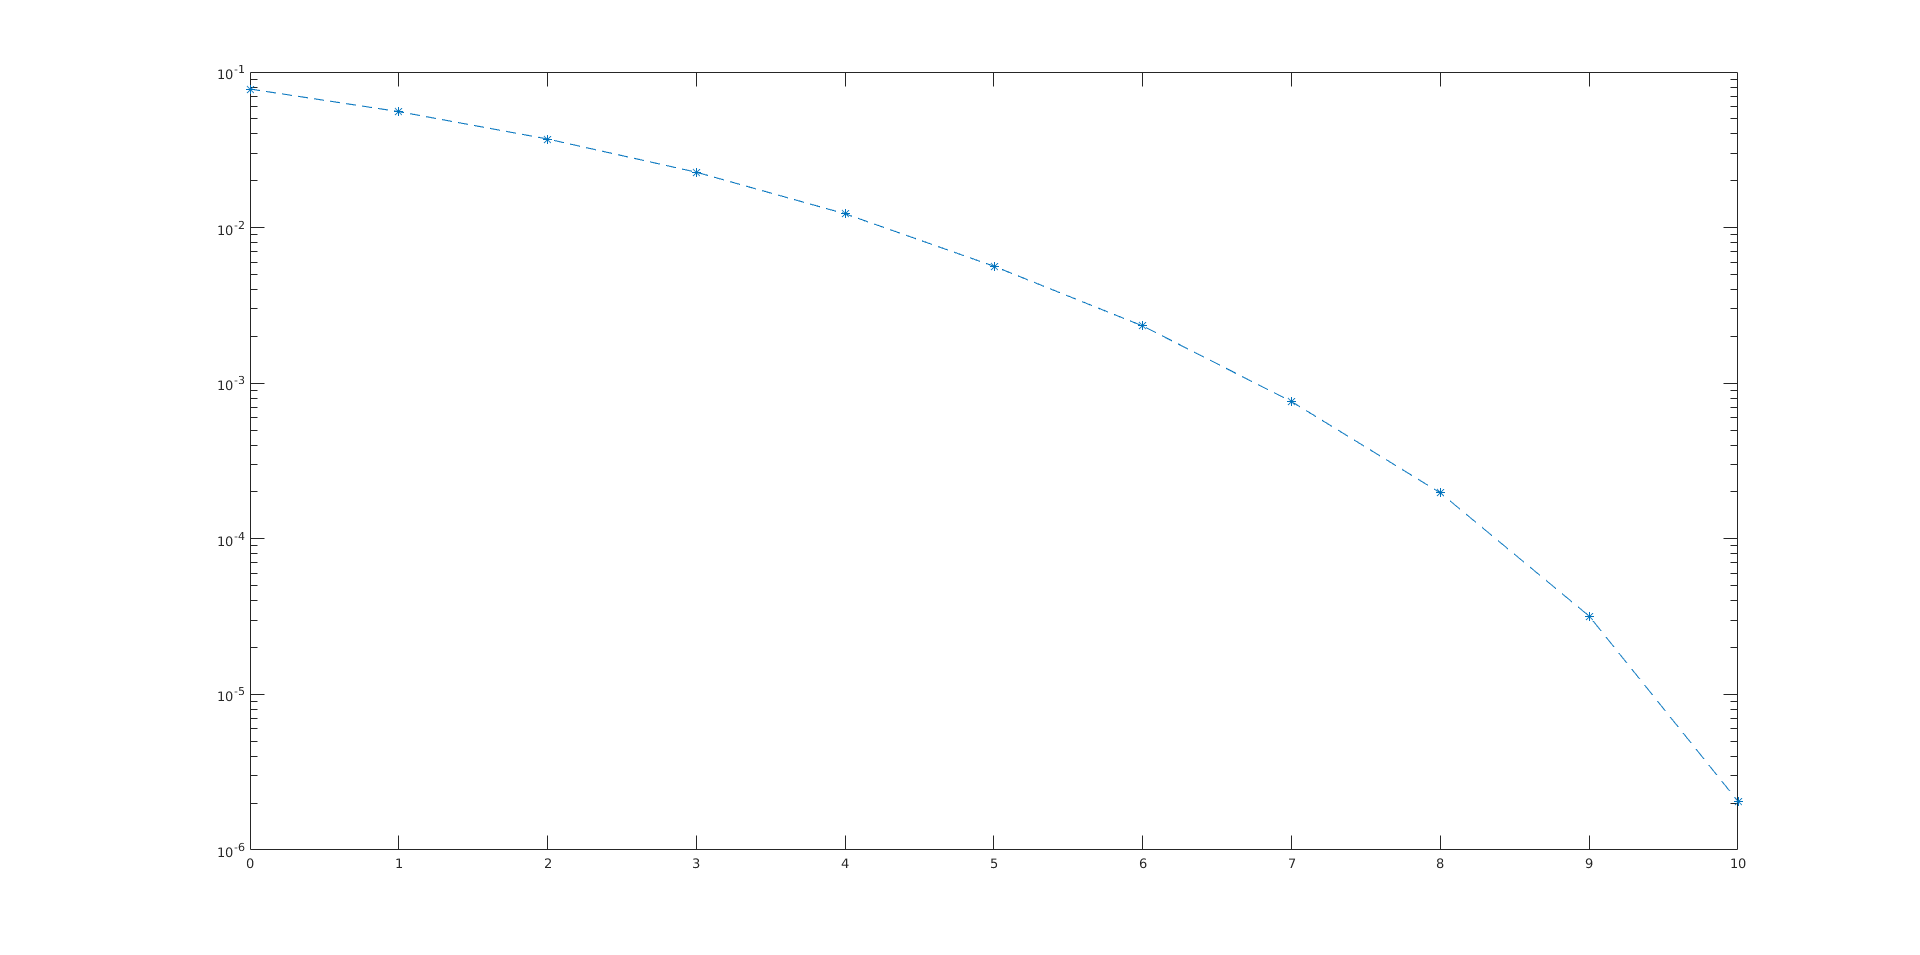
\includegraphics[width=\linewidth]{BERRC.png}
\caption{BER of Raised Cosine Filtered BPSK}
\label{fig:BERComp}
\end{figure}

\end{enumerate}


\section{Post Lab}
\label{sec:postlab}

Mueller and Muller Method

The error term is calculated using $e_n=(y_n*y_n-1)-(y_n*y_n-1)$,where $y_n$ is the current 
symbol sample and yn-1 is the sample from the previous symbol. This method uses one sample per 
symbol as opposed to three for Early Late gate. This method is sensitive to carrier offsets 
and carrier recovery must be done before Mueller and Muller timing recovery.



Gardner Method

The error term is calculated using $e_n=(y_n-y_n-2)y_n-1$, where spacing between $y_n$ and 
$y_n-2$ is T seconds and spacing between $y_n$ and $y_n-1$ is $T/2$ seconds.
This method uses two samples per symbol and is insensitive to carrier offsets.
Gardner error is most useful on symbol transitions, i.e. when the symbol switches polarities. 
The Gardner error is relatively small when the current and previous symbol have the same 
polarity.


Other methods

Running the transmitter and receiver off the same clock is the ideal solution but this is 
generally impossible in a wireless system. Another solution would be to transmit the clock 
signal along with the data but this method is inefficient because the clock signal consumes 
bandwidth and the transmitter power.


\section{Remarks}
\label{sec:remarks}


\end{document}